%卒業論文用雛形
\documentclass[a4j,12pt,oneside,openany]{jsbook}
% 英語なら以下を使う.
%\documentclass[a4j,12pt,oneside,openany,english]{jsbook}

\usepackage[dvipdfmx]{graphicx}
\usepackage{amssymb}
\usepackage{amsmath}
\usepackage{latexsym}

%jsbook を report っぽくするスタイルファイル
\usepackage{book2report}
%定理,補題,系,例題,証明などや英語用の定義がされています.
%自分なりにいじってください.
\usepackage{thesis}
% 具体的には以下のように定義されています.
% 英語の定理環境
%  \newtheorem{theorem}{Theorem}[chapter]
%  \newtheorem{lemma}{Lemma}[chapter]
%  \newtheorem{proposition}{Proposition}[chapter]
%  \newtheorem{corollary}{Corollary}[chapter]
%  \newtheorem{definition}{Definition}[chapter]
%  \newtheorem{example}{Example}[chapter]
%  \newtheorem{proof}{Proof}
% 日本語の定理環境
%  \newtheorem{theorem}{定理}[chapter]
%  \newtheorem{lemma}{補題}[chapter]
%  \newtheorem{proposition}{命題}[chapter]
%  \newtheorem{corollary}{系}[chapter]
%  \newtheorem{definition}{定義}[chapter]
%  \newtheorem{example}{例}[chapter]
%  \newtheorem{proof}{証明}
% 証明には番号をつけず,最後は Box で終わります.

% 英語で,見出しのフォントが気に入らなかったら
%\renewcommand{\headfont}{\bfseries}

% ページ数が少ないときはここを大きくしてごまかそう!!効果絶大!!
\renewcommand{\baselinestretch}{1.0}

\begin{document}
\appendix
\chapter{ニューラルネットワークの基礎}
\par
ニューラルネットワークは,動物の脳神経系を模倣した情報処理の数理的モデルである\cite{bib12, bib13, bib14}.
本節では,入力に対して確定的に出力が決まる階層型ニューラルネットワークの数理モデルについて説明を行う.

\par
階層型ニューラルネットワークは多層パーセプトロンとよばれ,単純パーセプトロンを層状に繋ぎあわせた構造をしている.
単純パーセプトロンはRosenblattが提案した情報処理モデルである\cite{bib15}.
図\ref{fig:a-neural-1}に例を示す.
\begin{figure}[t]
 \centering
 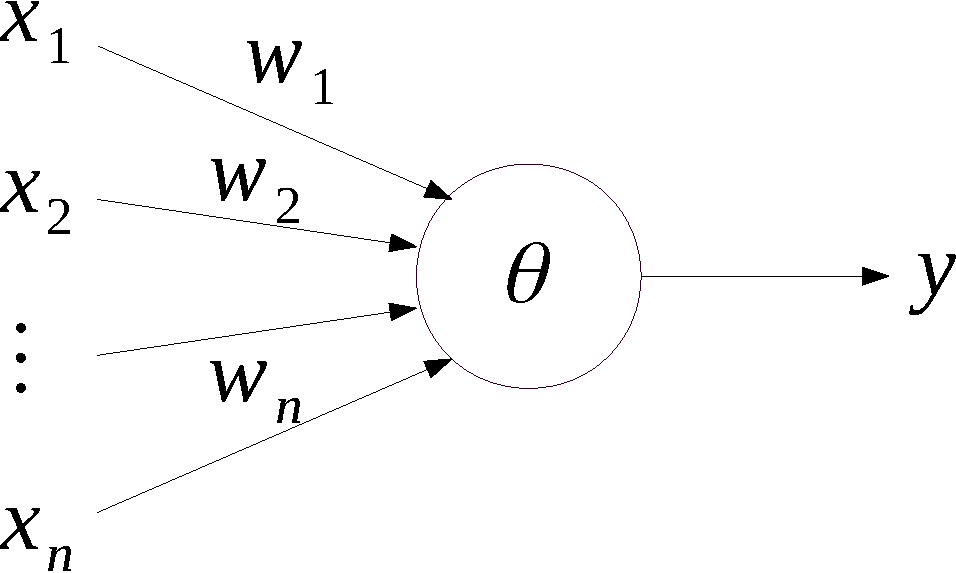
\includegraphics[keepaspectratio, width=50mm]
 {Graphics/appendix/neural1-crop.pdf}
 \caption{単純パーセプトロンの例}
 \label{fig:a-neural-1}
\end{figure}
単純パーセプトロンでは,多次元の入力$\bm{x} = (x_1, \ldots, x_n)\in\mathbb{R}^{n}$に対する出力$y\in\mathbb{R}$を以下のように計算する.
\begin{align}
 y &= a\bigg( \sum_{i=1}^{n}w_ix_i-\theta \bigg)\label{eq:a-neural-1}\\
 a(t) &= \left\{
 \begin{array}{ll}
  1 & \mbox{if }t \geq 0 \\
  0 & \mbox{otherwise}\label{eq:a-neural-2}
 \end{array}\right.
\end{align}
ただし,$w_i\in\mathbb{R}$は第$i$番目の入力要素$x_i$に対する結合の重みである.
$\theta\in\mathbb{R}$はしきい値である.
関数$a(\cdot)$は単純パーセプトロンの活性化関数や出力関数と呼ばれる.
ここで,常に$1$の値をとるダミー変数$x_0$を導入して,$x = (x_0, \ldots, x_n)$,$w = (w_0, \ldots, w_n)$とすれば,式(\ref{eq:a-neural-1})は
\begin{align}
 y = a\bigg( \sum_{i=0}^{n}w_ix_i \bigg) = a(\bm{w}^{\mathrm{T}}\bm{x})\label{eq:a-neural-3}
\end{align}
となる.
ただし,$w_0 = -\theta$である.

\par
図\ref{fig:a-neural-2}に4層からなる多層パーセプトロンの例を示す.
\begin{figure}[t]
 \centering
 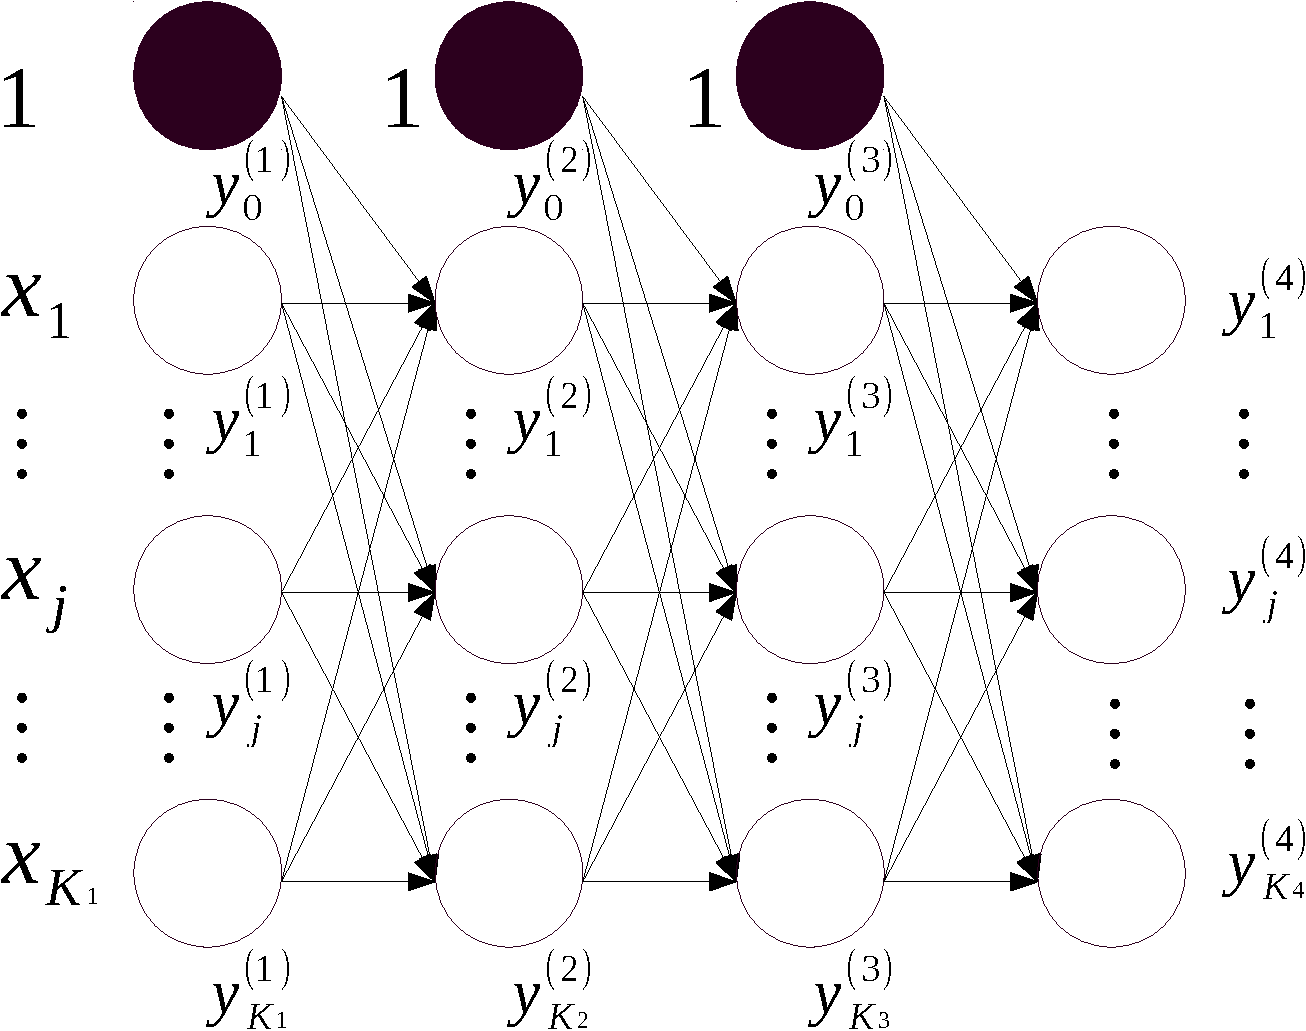
\includegraphics[keepaspectratio, width=100mm]
 {Graphics/appendix/neural2-crop.pdf}
 \caption{多層パーセプトロンの例}
 \label{fig:a-neural-2}
\end{figure}
この例では,入力層に入力された信号$x$は途中2つの中間層を経て出力層に伝播している.
各層の単純パーセプトロン(以下ノードと呼ぶ)では,式(\ref{eq:a-neural-1})に従って信号が変換される.
ただし,入力層のノードは入力信号をそのまま出力するので,$y_i^{(1)}=x_i$である.
多層パーセプトロンの第$n$層の第$k$ノードから第$n+1$層の第$j$ノードへの結合の重みを$w_{k, j}^{(n+1)}$とする.
ネットワークの中の結合の重みをすべてまとめて$W=\{w_{k, j}^{n}\}$と書くと,多層パーセプトロンの出力は$y=g(\bm{x},W)$のように入力ベクトルと結合の重みによって決まる.
また,Cybenkoは中間層の活性化関数が
\begin{align}
 a(t) = \left\{
 \begin{array}{ll}
  1 & \mbox{as }t \to \infty \\
  0 & \mbox{as }t \to -\infty\label{eq:a-neural-4}
 \end{array}\right.
\end{align}
の性質を持つ非線形の連続な単調増加関数であり,出力層の活性化関数が線形関数であるとき,中間層が1層の多層パーセプトロンによって任意の連続関数が関数$g$によって近似可能であることを示している\cite{bib16}.

\par
最後に,多層パーセプトロンの重みの学習方法のひとつである誤差逆伝播学習について説明する\cite{bib17}.
誤差逆伝播学習法では,ノードの活性化関数として微分可能な関数を用いる.
ここでは,式(\ref{eq:a-neural-5})のシグモイド関数を用いた場合の説明をする.
\begin{align}
 a(t) = \mbox{sig}(t) = \frac{1}{1+e^{-t}}\label{eq:a-neural-5}
\end{align}
多層パーセプトロンの層の数は$N$とし,学習用のデータとして入力$\bm{x}$と正解の出力$\bm{r}$を与える.
学習のための評価基準として,出力層での誤差評価,例えば二乗誤差を用いることにする.
\begin{align}
 E(W)=\frac{1}{2}\sum_{j=1}^{K_N}(r_j-y_j^{(N)})^2\label{eq:a-neural-5}
\end{align}
活性化関数は微分可能なものを仮定しているので,誤差評価$E(W)$への結合の重み$w_{k, j}^n$の寄与を$E(W)$の偏微分係数として計算することができる.
つまり,勾配降下法により,出力と正解のデータとの誤差が小さくなるように,すべての結合の重みを更新することができる.
例えば,確率的勾配降下法による結合の重みの更新は以下のようになる.
\begin{align}
 w_{k, j}^{(n+1)} & \gets w_{k, j}^{(n+1)} - \eta \frac{\partial E(W)}{\partial w_{k, j}^{(n+1)}}\nonumber\\
& = w_{k, j}^{(n+1)} - \eta \delta_j^{(n+1)}y_k^{(n)}\label{eq:a-neural-6}
\end{align}
ただし,$\eta$は学習率である.
式(\ref{eq:a-neural-6})の中にある$\delta_j^{(n+1)}$は以下の式で求められる.
\begin{align}
\delta_j^{(N)}& = -(r_j - y_j^{(N)}) y_j^{(N)} (1 - y_j^{(N)})\label{eq:a-neural-7}\\
\delta_j^{(n)}& = \bigg\{ \sum_{k=1}^{K_{n+1}}\delta_j^{(n+1)}w_{k, j}^{(n+1)} \bigg\} y_j^{(n)} (1 - y_j^{(n)})\label{eq:a-neural-8}
\end{align}
$\delta_j^{(n+1)}$の計算過程を見ると,出力層での誤差を前の層に伝播させていく形になっている.
このことが誤差逆伝播学習の名前の由来である.

\chapter{混合論理動的システム}
\par
 混合論理動的システム(以下MLDシステムと呼ぶ)モデルは
\begin{align}
 \begin{cases}
  x(k+1) = Ax(k)+B_1u(k)+B_2z(k)+B_3\delta(k)\\
  Cx(k)+D_1u(k)+D_2z(k)+D_3\delta(k)\leq D_4
 \end{cases}
\end{align}
で与えられる\cite{bib11}.
ここで,$x(k)\in\mathbb{R}^n$は状態,$u(k)\in\mathbb{R}^m$は入力,$z(k)\in\mathbb{R}^{l_1}$と$\delta(k)\in\{0,\ 1\}^{l_2}$は補助変数である.
また,$A\in\mathbb{R}^{n\times n}$,$B_1\in\mathbb{R}^{n\times m}$,$B_2\in\mathbb{R}^{n\times l_1}$,$B_3\in\mathbb{R}^{n\times l_2}$,$C\in\mathbb{R}^{q\times n}$,$D_1\in\mathbb{R}^{q\times m}$,$D_2\in\mathbb{R}^{q\times l_1}$,$D_3\in\mathbb{R}^{q\times l_2}$,$D_4\in\mathbb{R}^{q}$は定数行列である.
補助変数$\delta$は,このモデルの離散状態を表している.

\par
バイナリ変数と論理積,論理和,否定などの論理演算を含む命題論理は,バイナリ変数と四則演算からなる線形不等式で表現できる.
例えば,命題$i$の真偽を表す変数を論理変数と呼び,$X_i\in\{0,\ 1\}$で表す.
そして,$X_i$を命題「$\delta_i=1$である」と対応付け,$X_i=[\delta_i=1]$と表現することにする.
すると,各論理演算について以下の補題が成り立つ.
\lemma{}
\ 
\begin{enumerate}
 \item $[\delta_1=1] \lor [\delta_2=1]\ (=X_1 \lor X_2)$と$\delta_1+\delta_2\geq 1$は等価である.
 \item $[\delta_1=1] \land [\delta_2=1]\ (=X_1 \land X_2)$と$\delta_1=1$,$\delta_2=1$は等価である.
 \item $[\delta_1=1] \to [\delta_2=1]\ (=X_1 \to X_2)$と$\delta_1-\delta_2\leq 0$は等価である.
 \item $[\delta_1=1] \leftrightarrow [\delta_2=1]\ (=X_1 \leftrightarrow X_2)$と$\delta_1-\delta_2 = 0$は等価である.
 \item $[\delta_1=1] \oplus [\delta_2=1]\ (=X_1 \oplus X_2)$と$\delta_1+\delta_2 = 1$は等価である.
\end{enumerate}
ただし,$\lor$,$\land$,$\to$,$\leftrightarrow$,$\oplus$は,それぞれ,論理和,論理積,否定,含意,等価,排他的論理和である.

\par
最後に本論文で利用した,連続値変数を含む場合の論理条件の不等式表現について補題を示す.
\lemma{}
$\delta\in\{0,\ 1\}$をインデックス変数,$x\in\mathbb{R}^n$を連続値変数とする.
このとき,関数$h\ :\ \mathbb{R}^{n}\to\mathbb{R}$,$g\ :\ \mathbb{R}^{n}\to\mathbb{R}^{m}$に対して,有界集合$\mathbb{X}\subset\mathbb{R}^{n}$上で次の関係が成り立つ.
\begin{enumerate}
 \item $[\delta_1=1] \leftrightarrow [h(x)\geq 0]$は,つぎの線形不等式によって任意の精度で近似できる.
\begin{align}
  h_{\inf}(1-\delta)\leq h(x)\leq h_{\sup}(\delta-1)\epsilon
\end{align}
ただし,$h_{\inf}$,$h_{\sup}\in\mathbb{R}$はすべての$x\in\mathbb{X}$に対して$h_{\inf}\leq h(x)\leq h_{\sup}$を満たすものであり,$\epsilon\in\mathbb{R}_{++}$は任意に選ばれた十分小さい定数である.
 \item $z=\delta g(x)$はつぎの不等式と等価である.
\begin{align}
  g_{\inf}\delta\leq z\leq g_{\sup}\delta
\end{align}
\begin{align}
  g(x)-g_{\sup}(1-\delta)\leq z\leq g(x)-g_{\inf}(1-\delta)
\end{align}
\end{enumerate}
ただし,$g_{\inf}$,$g_{\sup}\in\mathbb{R}^{m}$はすべての$x\in\mathbb{X}$に対して$g_{\inf}\leq g(x)\leq g_{\sup}$を満たすベクトルである.
% \chapter{モデル予測制御}
% \par
% システムのダイナミクスが
% \begin{align}
%  \begin{cases}
%   x(k+1) = Ax(k)+Bu(k)\\
%   Cx(k)+Du(k) \leq E
%  \end{cases}
% \end{align}
% で与えられているとする.
% ここで,$x(k)\in\mathbb{R}^n$は状態,$u(k)\in\mathbb{R}^m$は入力である.
% また,$A\in\mathbb{R}^{n\times n}$,$B\in\mathbb{R}^{n\times m}$,$C\in\mathbb{R}^{q\times n}$,$D\in\mathbb{R}^{q\times m}$,$E\in\mathbb{R}^{q}$は定数行列である.
% このシステムに対して,つぎの有限時間最適制御問題を考える.





% \par
% モデル予測制御は現時点から有限区間内の制約条件がシステムのダイナミクスとなっている数理計画問題を解き,得られた有限区間の入力のうち初期入力の1ステップ分のみを制御入力として利用し,各時刻でこれを繰り返し行い制御する方法である.
% モデル予測制御は現時点から$T$ステップ先のシステムの状態量を数理計画問題を解くことで予測するため,有限区間の終端時刻$T$は予測ステップ数と呼ばれる.

% \par
% モデル予測制御には計算時間に関する課題がある.
% まず,モデル予測制御を実装するには各時刻でのシステムの状態を計測したら即座に最適制御問題を解いて制御入力を決定する必要がある.
% したがって,最適制御問題の数値解法は時刻の時間単位内に終わる必要がある.
\end{document}